\documentclass[letterpaper,11pt]{article}
\usepackage[utf8x]{inputenc}
\usepackage{enumerate}
\usepackage{enumitem}
\usepackage{fullpage}
\usepackage{amsmath}

\usepackage{pgf}
\usepackage{tikz}
\usepackage{circuitikz}
\usepackage[free-standing-units]{siunitx}

%opening
\title{Final Exam \\ Classical Mechanics \\ Physics 601 (Fall 2012)}
\date{Monday December 17, 2012, 9am}

\begin{document}

\maketitle

\paragraph*{Instructions}
\begin{itemize}
 \item This exam is governed by \textbf{William \& Mary Honor Code}.
 \item This exam is to be completed \textbf{individually}.
 \item This exam is `open notes:' you are allowed to use the textbook, the posted lecture notes and homework solutions, and your personal notes.
 \item Carefully explain each step in your answer.
 \item Calculators are not needed for this exam.
 \item Write your \textbf{name on every page}.
 \item Write your responses on \textbf{single-sided} letter paper.
\end{itemize}

\pagebreak

\paragraph*{Lagrangian Mechanics and Rigid Bodies}
\begin{enumerate}
 \item Describe the motion of a uniform solid sphere with mass $M$ and radius $R$ that is rolling without slipping on a horizontal turntable rotating with a constant angular velocity $\Omega$.\footnotemark{}
 \footnotetext{This question was inspired by a real-world (and late-night) `problem' involving a rotating cheese platter, and the ball from a foosball table.}
 \begin{center}
  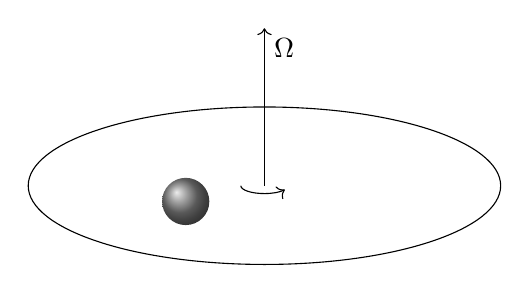
\begin{tikzpicture}
   \draw (0,0) ellipse (3 and 1);
   \draw (-0.3,0)[->] arc (180:330:0.3 and 0.1);
   \draw (0,0)[->] -- (0,2) node[very near end,right] {$\Omega$};
   \shade[ball color=gray] (-1,-0.2) circle (.3);
  \end{tikzpicture}
 \end{center}
 \begin{enumerate}
  \item Determine the inertia tensor $I$ of the sphere.  What are the principal axes? [5 points]
  \item Determine the Lagrangian using the Cartesian coordinates $\vec{r} = x\hat{e}_1 + y\hat{e}_2$ of the center of the sphere and the Euler angles $\alpha$, $\beta$ and $\gamma$. [5 points]
  \item Determine the constraints for this problem.  Show whether they are holonomic.  You should find constraints of the form
  \begin{eqnarray*}
   u \equiv \dot{x} + a y = b \omega_y \quad & \hbox{or} & \quad dx + a y dt = b \omega_y dt, \\
   v \equiv \dot{y} - a x = - b \omega_x \quad & \hbox{or} & \quad dy - a x dt = - b \omega_x dt,
  \end{eqnarray*}
  for specific constants $a$ and $b$ that you will determine (and where $\omega_i dt$ includes the dependence on $d\alpha$, $d\beta$ and $d\gamma$). [10 points]
  \item Introduce Lagrange multipliers and write the equations of motion.\footnotemark{}  What is the interpretation of the Lagrange multipliers? [10 points]
  \footnotetext{For partial credit, use the undetermined constants $a$ and $b$ in the constraints.}
  \item Identify the cyclic coordinate and interpret the constant of motion. [5 points]
  \item Using some tricky algebra that you do not need to demonstrate, one can eliminate the angles $\alpha$, $\beta$ and $\gamma$, and in particular one finds for the Lagrange multipliers
  \begin{eqnarray*}
   \lambda_1 & = & -\frac{I}{R^2}\dot{u} = -\frac{I}{R^2} (\ddot{x} + a \dot{y}), \\
   \lambda_2 & = & -\frac{I}{R^2}\dot{v} = -\frac{I}{R^2} (\ddot{y} - a \dot{x}).
  \end{eqnarray*}
  Using these expressions and the equations for $x$ and $y$, show that circles are solutions:
  \begin{eqnarray*}
   x(t) & = & x_c + A \cos \rho (t - t_0), \\
   y(t) & = & y_c + A \sin \rho (t - t_0),
  \end{eqnarray*}
  with integration constants $x_c$, $y_c$, $A$ and $t_0$ determined by the initial conditions.  What is the frequency $\rho$ with which the sphere will describe these circles? [10 points]
  \item This problem has a close analog in the circular motion of a charged particle in a uniform magnetic field.  Explain where the similarity comes from. [5 points]
 \end{enumerate}
\end{enumerate}


\paragraph*{Hamiltonian Mechanics}
\begin{enumerate}[resume]
 \item A particle with mass $m$ is moving in periodic motion in one dimension under the influence of a potential $V(x) = k|x|$.  Use action-angle variables to find the frequency of the motion as a function of the particle energy $E$. [20 points]
 \begin{center}
  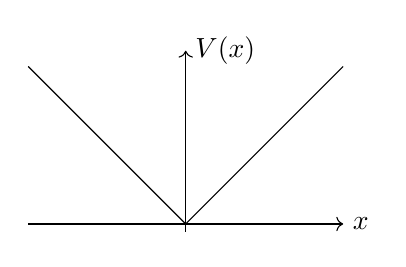
\begin{tikzpicture}
   \draw (-2,0)[->] -- (2,0) node[right] {$x$};
   \draw (0,-0.1)[->] -- (0,2.2) node[right] {$V(x)$};
   \draw (-2,2) -- (0,0) -- (2,2);
  \end{tikzpicture}
 \end{center}
\end{enumerate}

\begin{enumerate}[resume]
 \item In the case of a time-dependent Hamiltonian $H\left(p,q;\lambda(t)\right)$ where the time-dependence is due to a parameter $\lambda$ that slowly varies in time, the action $J$ belongs to a class of observables known as \emph{adiabatic invariants}.  The change in $\lambda$ is said to be adiabatic if the change $\Delta\lambda$ is slow compared to the period of the motion, or
 \begin{equation*}
  |\Delta\lambda| = |\dot\lambda| \Delta t = |\dot\lambda| \frac{2\pi}{\omega} \ll |\lambda|.
 \end{equation*}
 For changes in the parameter $\lambda$ that satisfy this \emph{adiabatic condition} the action $J$ is conserved.

 At the first international Solvay congress in 1911, the following question was posed: how would the energy of a simple pendulum change if the length $\ell$ is changed slowly.  Model the simple pendulum with small amplitude as a harmonic oscillator $H\left(p,q;\omega(t)\right)$, and determine how the following quantities change when the length is \emph{doubled} adiabatically: [10 points]
 \begin{itemize}
  \item the total energy $E$ of the harmonic oscillator,
  \item the amplitude $\theta_{max}$ of the pendulum.
 \end{itemize}
\end{enumerate}

\paragraph*{Small Oscillations}
\begin{enumerate}[resume]
 \item Consider the following coupled $LC$ circuit where $I_{1,2} = dQ_{1,2}/dt$ is the current flowing in a loop of the circuit, $L$ is the inductance of the inductor, and $C$ is the capacitance of the capacitor.  By analogy to mechanical oscillators, the inductance plays the role of an inertial mass, the capacitance plays the role of a spring constant.  The kinetic energy in an inductor is $\frac{1}{2} L I^2$, the potential energy in a capacitor is $\frac{1}{2 C} Q^2$.  The voltage across an inductor is $L \frac{d L}{d t}$, the voltage across a capacitor is $Q/C$.
 \begin{center}
  \begin{circuitikz}
   \draw (0,3) to (4,3);
   \draw (0,0) to[L, i=$I_1$, l=$L$] (0,3);
   \draw (0,0) to[C, l=$C$] (2,0);
   \draw (2,0) to[C, l=$C$] (4,0);
   \draw (4,0) to[L, i=$I_2$, l=$L$] (4,3);
   \draw (2,0) to (2,1);
   \draw (2,3) to[C, l=$C$] (2,1);
  \end{circuitikz}
 \end{center}
 \begin{enumerate}
  \item Determine the Lagrangian for this circuit, and show that the correct Kirchhoff equations can indeed be derived. [10 points]
  \item Treating the Lagrangian\footnotemark{} as a small oscillations problem, what are the frequencies of oscillation and the normal modes for this circuit when the currents and charges are small? [10 points]
  \footnotetext{For partial credit, use this \emph{incorrect} Lagrangian $L(I_1,I_2,Q_1,Q_2) = \frac{1}{2} L (I_1^2 + I_2^2) - \frac{1}{2 C} \left(Q_1 + Q_2\right)^2$}
 \end{enumerate}
\end{enumerate}


\end{document}
